%! TEX encoding = utf8
\chapter{Laboratorium}

\section{Określenie wartości pomiaru temperatury w punkcie pracy}

W celu określenia wartości pomiaru temperatury w punkcie pracy ustawiono moc wentylatora  $W1 = 50\%$,a moc grzałki $G1 = 25\%$.
Po czasie około 8 minut temperatura odczytywana przez czujnik temperatury zaczeła się stabilizować  na poziomie  $T1 = 30,93^{\circ} C$.

Niestety z powodu ciągłego ruchu powietrza związanego z przemieszczaniem się osób w sali i dużej ilości tych osób wpływających na temperaturę sali oraz czułość stanowiska pomiarowego temperatura odczytywana przez czujnik zaczeła odbiegać i lekko oscylować wokół tej temperatury.

\begin{figure}[H]
\centering
% This file was created by matlab2tikz.
%
%The latest updates can be retrieved from
%  http://www.mathworks.com/matlabcentral/fileexchange/22022-matlab2tikz-matlab2tikz
%where you can also make suggestions and rate matlab2tikz.
%
\definecolor{mycolor1}{rgb}{0.00000,0.44700,0.74100}%
%
\begin{tikzpicture}

\begin{axis}[%
width=4.521in,
height=3.566in,
at={(0.758in,0.481in)},
scale only axis,
xmin=0,
xmax=450,
xlabel style={font=\color{white!15!black}},
xlabel={k},
ymin=25,
ymax=31,
ylabel style={font=\color{white!15!black}},
ylabel={$\text{T[}^\circ\text{C]}$},
axis background/.style={fill=white}
]
\addplot[const plot, color=mycolor1, forget plot] table[row sep=crcr] {%
1	25.12\\
2	25.12\\
3	25.18\\
4	25.25\\
5	25.37\\
6	25.43\\
7	25.5\\
8	25.62\\
9	25.68\\
10	25.75\\
11	25.81\\
12	25.87\\
13	26\\
14	26.06\\
15	26.12\\
16	26.18\\
17	26.25\\
18	26.31\\
19	26.43\\
20	26.5\\
21	26.56\\
22	26.62\\
23	26.68\\
24	26.68\\
25	26.81\\
26	26.81\\
27	26.87\\
28	26.93\\
29	27\\
30	27.06\\
31	27.12\\
32	27.18\\
33	27.18\\
34	27.25\\
35	27.31\\
36	27.37\\
37	27.37\\
38	27.43\\
39	27.5\\
40	27.5\\
41	27.56\\
42	27.62\\
43	27.62\\
44	27.68\\
45	27.68\\
46	27.75\\
47	27.81\\
48	27.81\\
49	27.87\\
50	27.87\\
51	27.93\\
52	28\\
53	28\\
54	28\\
55	28.06\\
56	28.06\\
57	28.12\\
58	28.12\\
59	28.18\\
60	28.18\\
61	28.25\\
62	28.25\\
63	28.25\\
64	28.31\\
65	28.37\\
66	28.37\\
67	28.37\\
68	28.43\\
69	28.43\\
70	28.5\\
71	28.5\\
72	28.5\\
73	28.56\\
74	28.56\\
75	28.56\\
76	28.62\\
77	28.62\\
78	28.68\\
79	28.68\\
80	28.68\\
81	28.75\\
82	28.75\\
83	28.81\\
84	28.81\\
85	28.81\\
86	28.87\\
87	28.87\\
88	28.93\\
89	28.93\\
90	29\\
91	29\\
92	29\\
93	29\\
94	29.06\\
95	29.06\\
96	29.06\\
97	29.12\\
98	29.12\\
99	29.12\\
100	29.12\\
101	29.18\\
102	29.18\\
103	29.18\\
104	29.25\\
105	29.25\\
106	29.25\\
107	29.25\\
108	29.31\\
109	29.31\\
110	29.31\\
111	29.31\\
112	29.37\\
113	29.31\\
114	29.37\\
115	29.37\\
116	29.37\\
117	29.43\\
118	29.43\\
119	29.43\\
120	29.5\\
121	29.5\\
122	29.5\\
123	29.5\\
124	29.5\\
125	29.56\\
126	29.56\\
127	29.56\\
128	29.56\\
129	29.56\\
130	29.56\\
131	29.62\\
132	29.62\\
133	29.62\\
134	29.62\\
135	29.62\\
136	29.62\\
137	29.62\\
138	29.62\\
139	29.68\\
140	29.68\\
141	29.68\\
142	29.68\\
143	29.75\\
144	29.75\\
145	29.75\\
146	29.75\\
147	29.75\\
148	29.75\\
149	29.75\\
150	29.75\\
151	29.75\\
152	29.75\\
153	29.75\\
154	29.81\\
155	29.81\\
156	29.81\\
157	29.81\\
158	29.81\\
159	29.81\\
160	29.81\\
161	29.87\\
162	29.87\\
163	29.87\\
164	29.87\\
165	29.87\\
166	29.87\\
167	29.93\\
168	29.93\\
169	29.93\\
170	29.93\\
171	29.93\\
172	29.93\\
173	29.93\\
174	29.93\\
175	30\\
176	29.93\\
177	30\\
178	30\\
179	30\\
180	30\\
181	30\\
182	30\\
183	30\\
184	30\\
185	30\\
186	30.06\\
187	30.06\\
188	30.06\\
189	30.06\\
190	30.06\\
191	30.06\\
192	30.06\\
193	30.06\\
194	30.06\\
195	30.06\\
196	30.06\\
197	30.06\\
198	30.06\\
199	30.06\\
200	30.06\\
201	30.06\\
202	30.12\\
203	30.12\\
204	30.12\\
205	30.12\\
206	30.12\\
207	30.12\\
208	30.12\\
209	30.18\\
210	30.18\\
211	30.18\\
212	30.18\\
213	30.18\\
214	30.18\\
215	30.18\\
216	30.18\\
217	30.18\\
218	30.25\\
219	30.25\\
220	30.25\\
221	30.25\\
222	30.25\\
223	30.25\\
224	30.25\\
225	30.31\\
226	30.25\\
227	30.25\\
228	30.31\\
229	30.31\\
230	30.25\\
231	30.31\\
232	30.31\\
233	30.31\\
234	30.31\\
235	30.31\\
236	30.31\\
237	30.31\\
238	30.31\\
239	30.31\\
240	30.31\\
241	30.31\\
242	30.37\\
243	30.37\\
244	30.37\\
245	30.37\\
246	30.37\\
247	30.43\\
248	30.43\\
249	30.43\\
250	30.43\\
251	30.43\\
252	30.43\\
253	30.43\\
254	30.43\\
255	30.43\\
256	30.5\\
257	30.5\\
258	30.5\\
259	30.5\\
260	30.5\\
261	30.56\\
262	30.56\\
263	30.56\\
264	30.56\\
265	30.56\\
266	30.62\\
267	30.56\\
268	30.62\\
269	30.56\\
270	30.56\\
271	30.56\\
272	30.56\\
273	30.56\\
274	30.56\\
275	30.56\\
276	30.56\\
277	30.56\\
278	30.56\\
279	30.56\\
280	30.56\\
281	30.56\\
282	30.56\\
283	30.56\\
284	30.56\\
285	30.56\\
286	30.56\\
287	30.62\\
288	30.62\\
289	30.56\\
290	30.56\\
291	30.62\\
292	30.62\\
293	30.62\\
294	30.62\\
295	30.62\\
296	30.62\\
297	30.62\\
298	30.62\\
299	30.62\\
300	30.62\\
301	30.62\\
302	30.62\\
303	30.62\\
304	30.62\\
305	30.62\\
306	30.62\\
307	30.62\\
308	30.62\\
309	30.62\\
310	30.62\\
311	30.68\\
312	30.68\\
313	30.62\\
314	30.68\\
315	30.68\\
316	30.68\\
317	30.68\\
318	30.68\\
319	30.68\\
320	30.68\\
321	30.68\\
322	30.68\\
323	30.68\\
324	30.68\\
325	30.68\\
326	30.68\\
327	30.68\\
328	30.68\\
329	30.68\\
330	30.68\\
331	30.68\\
332	30.68\\
333	30.68\\
334	30.68\\
335	30.68\\
336	30.68\\
337	30.68\\
338	30.68\\
339	30.68\\
340	30.68\\
341	30.68\\
342	30.68\\
343	30.68\\
344	30.68\\
345	30.75\\
346	30.75\\
347	30.75\\
348	30.75\\
349	30.75\\
350	30.75\\
351	30.75\\
352	30.81\\
353	30.75\\
354	30.75\\
355	30.81\\
356	30.75\\
357	30.81\\
358	30.81\\
359	30.81\\
360	30.81\\
361	30.81\\
362	30.81\\
363	30.81\\
364	30.75\\
365	30.81\\
366	30.75\\
367	30.81\\
368	30.81\\
369	30.81\\
370	30.81\\
371	30.81\\
372	30.81\\
373	30.81\\
374	30.81\\
375	30.81\\
376	30.87\\
377	30.87\\
378	30.87\\
379	30.87\\
380	30.87\\
381	30.93\\
382	30.93\\
383	30.93\\
384	30.93\\
385	30.93\\
386	30.93\\
387	30.93\\
388	30.93\\
389	30.93\\
390	30.93\\
391	30.93\\
392	30.87\\
393	30.87\\
394	30.87\\
395	30.87\\
396	30.87\\
397	30.87\\
398	30.87\\
399	30.87\\
400	30.87\\
401	30.87\\
402	30.87\\
403	30.87\\
404	30.87\\
405	30.87\\
406	30.87\\
407	30.87\\
408	30.87\\
409	30.87\\
410	30.87\\
411	30.87\\
412	30.87\\
413	30.87\\
414	30.87\\
415	30.87\\
416	30.87\\
417	30.87\\
418	30.87\\
419	30.87\\
420	30.93\\
421	30.93\\
422	30.93\\
423	30.93\\
424	30.93\\
425	30.93\\
426	30.87\\
427	30.93\\
428	30.93\\
429	30.87\\
430	30.93\\
431	30.93\\
432	30.93\\
433	30.93\\
434	30.93\\
435	30.93\\
436	30.93\\
437	30.93\\
438	30.93\\
439	30.93\\
440	30.93\\
441	30.93\\
442	30.93\\
443	30.93\\
444	31\\
445	30.93\\
446	30.93\\
447	30.93\\
448	30.93\\
449	30.93\\
450	30.93\\
};
\end{axis}
\end{tikzpicture}%
\caption{Pomiar temperatury w punkcie pracy}
\end{figure}

\section{Wyznaczenie odpowiedzi skokowych}

Doprowadziliśmy układ do stanu stabilnego dla 7 różnych wartości sterowania: $U = 20$, $U = 30$, $U = 40$, $U = 50$, $U = 60$, $U = 70$, $U = 80$.

\begin{figure}[H]
\centering
% This file was created by matlab2tikz.
%
%The latest updates can be retrieved from
%  http://www.mathworks.com/matlabcentral/fileexchange/22022-matlab2tikz-matlab2tikz
%where you can also make suggestions and rate matlab2tikz.
%
\definecolor{mycolor1}{rgb}{0.00000,0.44700,0.74100}%
\definecolor{mycolor2}{rgb}{0.85000,0.32500,0.09800}%
\definecolor{mycolor3}{rgb}{0.92900,0.69400,0.12500}%
%
\begin{tikzpicture}

\begin{axis}[%
width=4.521in,
height=3.566in,
at={(0.758in,0.481in)},
scale only axis,
xmin=0,
xmax=350,
xlabel style={font=\color{white!15!black}},
xlabel={k},
ymin=28,
ymax=34,
ylabel style={font=\color{white!15!black}},
ylabel={$\text{T[}^\circ\text{C]}$},
axis background/.style={fill=white}
]
\addplot[const plot, color=mycolor1, forget plot] table[row sep=crcr] {%
1	28.18\\
2	28.18\\
3	28.18\\
4	28.18\\
5	28.12\\
6	28.12\\
7	28.12\\
8	28.12\\
9	28.12\\
10	28.12\\
11	28.12\\
12	28.12\\
13	28.06\\
14	28.12\\
15	28.12\\
16	28.12\\
17	28.12\\
18	28.18\\
19	28.18\\
20	28.18\\
21	28.18\\
22	28.25\\
23	28.25\\
24	28.25\\
25	28.25\\
26	28.31\\
27	28.31\\
28	28.31\\
29	28.37\\
30	28.37\\
31	28.43\\
32	28.43\\
33	28.43\\
34	28.5\\
35	28.56\\
36	28.56\\
37	28.62\\
38	28.62\\
39	28.68\\
40	28.68\\
41	28.68\\
42	28.75\\
43	28.75\\
44	28.81\\
45	28.87\\
46	28.87\\
47	28.87\\
48	28.93\\
49	28.93\\
50	29\\
51	29.06\\
52	29.06\\
53	29.12\\
54	29.18\\
55	29.18\\
56	29.25\\
57	29.25\\
58	29.31\\
59	29.31\\
60	29.37\\
61	29.37\\
62	29.37\\
63	29.37\\
64	29.43\\
65	29.43\\
66	29.5\\
67	29.5\\
68	29.5\\
69	29.56\\
70	29.56\\
71	29.56\\
72	29.62\\
73	29.62\\
74	29.62\\
75	29.62\\
76	29.62\\
77	29.62\\
78	29.62\\
79	29.62\\
80	29.62\\
81	29.62\\
82	29.62\\
83	29.62\\
84	29.62\\
85	29.62\\
86	29.62\\
87	29.62\\
88	29.62\\
89	29.68\\
90	29.68\\
91	29.68\\
92	29.68\\
93	29.75\\
94	29.75\\
95	29.75\\
96	29.75\\
97	29.81\\
98	29.81\\
99	29.81\\
100	29.81\\
101	29.81\\
102	29.81\\
103	29.87\\
104	29.87\\
105	29.87\\
106	29.87\\
107	29.87\\
108	29.87\\
109	29.87\\
110	29.93\\
111	29.93\\
112	29.87\\
113	29.87\\
114	29.87\\
115	29.87\\
116	29.93\\
117	29.87\\
118	29.93\\
119	29.93\\
120	29.93\\
121	29.93\\
122	29.93\\
123	29.93\\
124	29.93\\
125	29.87\\
126	29.87\\
127	29.93\\
128	29.93\\
129	29.93\\
130	29.93\\
131	29.93\\
132	29.93\\
133	30\\
134	30\\
135	30\\
136	30\\
137	30\\
138	30\\
139	30\\
140	30\\
141	30\\
142	30.06\\
143	30.06\\
144	30.06\\
145	30.06\\
146	30.06\\
147	30.12\\
148	30.12\\
149	30.12\\
150	30.12\\
151	30.12\\
152	30.12\\
153	30.12\\
154	30.12\\
155	30.12\\
156	30.18\\
157	30.18\\
158	30.18\\
159	30.18\\
160	30.18\\
161	30.18\\
162	30.25\\
163	30.25\\
164	30.25\\
165	30.25\\
166	30.25\\
167	30.25\\
168	30.31\\
169	30.31\\
170	30.31\\
171	30.31\\
172	30.31\\
173	30.31\\
174	30.37\\
175	30.37\\
176	30.37\\
177	30.37\\
178	30.37\\
179	30.37\\
180	30.43\\
181	30.43\\
182	30.43\\
183	30.43\\
184	30.43\\
185	30.43\\
186	30.43\\
187	30.37\\
188	30.43\\
189	30.37\\
190	30.37\\
191	30.37\\
192	30.37\\
193	30.37\\
194	30.37\\
195	30.37\\
196	30.37\\
197	30.37\\
198	30.37\\
199	30.37\\
200	30.37\\
201	30.37\\
202	30.37\\
203	30.37\\
204	30.37\\
205	30.37\\
206	30.37\\
207	30.37\\
208	30.37\\
209	30.37\\
210	30.37\\
211	30.37\\
212	30.37\\
213	30.37\\
214	30.37\\
215	30.37\\
216	30.37\\
217	30.37\\
218	30.37\\
219	30.37\\
220	30.43\\
221	30.43\\
222	30.43\\
223	30.43\\
224	30.43\\
225	30.43\\
226	30.43\\
227	30.43\\
228	30.43\\
229	30.43\\
230	30.43\\
231	30.43\\
232	30.43\\
233	30.37\\
234	30.37\\
235	30.37\\
236	30.37\\
237	30.43\\
238	30.43\\
239	30.43\\
240	30.43\\
241	30.43\\
242	30.43\\
243	30.43\\
244	30.43\\
245	30.43\\
246	30.43\\
247	30.43\\
248	30.5\\
249	30.5\\
250	30.5\\
251	30.5\\
252	30.5\\
253	30.5\\
254	30.5\\
255	30.5\\
256	30.5\\
257	30.5\\
258	30.5\\
259	30.5\\
260	30.5\\
261	30.5\\
262	30.5\\
263	30.5\\
264	30.5\\
265	30.56\\
266	30.5\\
267	30.5\\
268	30.5\\
269	30.5\\
270	30.5\\
271	30.5\\
272	30.5\\
273	30.5\\
274	30.5\\
275	30.5\\
276	30.5\\
277	30.5\\
278	30.5\\
279	30.5\\
280	30.5\\
281	30.5\\
282	30.5\\
283	30.5\\
284	30.5\\
285	30.5\\
286	30.5\\
287	30.56\\
288	30.56\\
289	30.56\\
290	30.56\\
291	30.56\\
292	30.56\\
293	30.56\\
294	30.56\\
295	30.56\\
296	30.56\\
297	30.56\\
298	30.56\\
299	30.56\\
300	30.56\\
301	30.5\\
302	30.5\\
303	30.5\\
304	30.5\\
305	30.5\\
306	30.5\\
307	30.43\\
308	30.43\\
309	30.43\\
310	30.43\\
311	30.43\\
312	30.43\\
313	30.43\\
314	30.43\\
315	30.37\\
316	30.37\\
317	30.37\\
318	30.37\\
319	30.37\\
320	30.37\\
321	30.37\\
322	30.37\\
323	30.37\\
324	30.37\\
325	30.37\\
326	30.43\\
327	30.43\\
328	30.43\\
329	30.5\\
330	30.43\\
331	30.5\\
332	30.5\\
333	30.5\\
334	30.56\\
335	30.56\\
336	30.56\\
337	30.56\\
338	30.56\\
339	30.56\\
340	30.56\\
341	30.56\\
342	30.62\\
343	30.62\\
344	30.62\\
345	30.62\\
346	30.62\\
347	30.62\\
348	30.62\\
349	30.62\\
350	30.62\\
};
\addplot[const plot, color=mycolor2, forget plot] table[row sep=crcr] {%
1	28.12\\
2	28.18\\
3	28.18\\
4	28.18\\
5	28.18\\
6	28.18\\
7	28.18\\
8	28.18\\
9	28.18\\
10	28.18\\
11	28.18\\
12	28.18\\
13	28.18\\
14	28.18\\
15	28.18\\
16	28.18\\
17	28.18\\
18	28.18\\
19	28.18\\
20	28.25\\
21	28.25\\
22	28.25\\
23	28.31\\
24	28.31\\
25	28.31\\
26	28.37\\
27	28.37\\
28	28.43\\
29	28.5\\
30	28.5\\
31	28.56\\
32	28.56\\
33	28.62\\
34	28.62\\
35	28.68\\
36	28.75\\
37	28.81\\
38	28.81\\
39	28.87\\
40	28.93\\
41	28.93\\
42	29\\
43	29.06\\
44	29.06\\
45	29.06\\
46	29.12\\
47	29.18\\
48	29.18\\
49	29.25\\
50	29.31\\
51	29.31\\
52	29.31\\
53	29.37\\
54	29.43\\
55	29.43\\
56	29.5\\
57	29.5\\
58	29.56\\
59	29.62\\
60	29.62\\
61	29.68\\
62	29.68\\
63	29.75\\
64	29.75\\
65	29.81\\
66	29.81\\
67	29.81\\
68	29.87\\
69	29.87\\
70	29.93\\
71	29.93\\
72	30\\
73	30\\
74	30.06\\
75	30.06\\
76	30.12\\
77	30.12\\
78	30.18\\
79	30.18\\
80	30.18\\
81	30.25\\
82	30.31\\
83	30.31\\
84	30.31\\
85	30.37\\
86	30.37\\
87	30.37\\
88	30.37\\
89	30.43\\
90	30.43\\
91	30.43\\
92	30.43\\
93	30.43\\
94	30.5\\
95	30.5\\
96	30.5\\
97	30.5\\
98	30.5\\
99	30.56\\
100	30.62\\
101	30.62\\
102	30.62\\
103	30.62\\
104	30.68\\
105	30.68\\
106	30.75\\
107	30.75\\
108	30.81\\
109	30.81\\
110	30.87\\
111	30.87\\
112	30.87\\
113	30.93\\
114	30.93\\
115	31\\
116	31\\
117	31.06\\
118	31\\
119	31.06\\
120	31.06\\
121	31\\
122	31\\
123	31\\
124	31.06\\
125	31\\
126	31\\
127	31.06\\
128	31.06\\
129	31.06\\
130	31.06\\
131	31.06\\
132	31.12\\
133	31.12\\
134	31.12\\
135	31.12\\
136	31.18\\
137	31.18\\
138	31.18\\
139	31.18\\
140	31.18\\
141	31.18\\
142	31.25\\
143	31.25\\
144	31.25\\
145	31.25\\
146	31.25\\
147	31.31\\
148	31.31\\
149	31.31\\
150	31.31\\
151	31.31\\
152	31.37\\
153	31.37\\
154	31.37\\
155	31.43\\
156	31.43\\
157	31.5\\
158	31.5\\
159	31.5\\
160	31.5\\
161	31.5\\
162	31.5\\
163	31.5\\
164	31.5\\
165	31.56\\
166	31.56\\
167	31.56\\
168	31.56\\
169	31.56\\
170	31.56\\
171	31.56\\
172	31.56\\
173	31.62\\
174	31.62\\
175	31.62\\
176	31.62\\
177	31.62\\
178	31.68\\
179	31.68\\
180	31.68\\
181	31.62\\
182	31.68\\
183	31.68\\
184	31.68\\
185	31.68\\
186	31.68\\
187	31.68\\
188	31.68\\
189	31.68\\
190	31.68\\
191	31.62\\
192	31.62\\
193	31.68\\
194	31.68\\
195	31.68\\
196	31.68\\
197	31.68\\
198	31.68\\
199	31.68\\
200	31.68\\
201	31.68\\
202	31.68\\
203	31.62\\
204	31.68\\
205	31.68\\
206	31.68\\
207	31.68\\
208	31.68\\
209	31.68\\
210	31.75\\
211	31.75\\
212	31.75\\
213	31.75\\
214	31.75\\
215	31.75\\
216	31.81\\
217	31.81\\
218	31.81\\
219	31.81\\
220	31.81\\
221	31.81\\
222	31.87\\
223	31.87\\
224	31.87\\
225	31.87\\
226	31.87\\
227	31.93\\
228	31.93\\
229	31.93\\
230	31.93\\
231	32\\
232	32\\
233	32\\
234	32\\
235	32\\
236	32\\
237	32\\
238	32\\
239	32\\
240	32\\
241	32\\
242	32\\
243	32\\
244	32.06\\
245	32.06\\
246	32.06\\
247	32.06\\
248	32.06\\
249	32.06\\
250	32.06\\
251	32.06\\
252	32\\
253	32\\
254	32\\
255	32\\
256	32\\
257	32\\
258	32\\
259	32\\
260	32\\
261	32\\
262	32\\
263	32\\
264	32\\
265	31.93\\
266	32\\
267	32\\
268	32\\
269	32\\
270	32\\
271	32\\
272	32\\
273	31.93\\
274	31.93\\
275	32\\
276	31.93\\
277	31.93\\
278	31.93\\
279	31.93\\
280	31.93\\
281	31.93\\
282	31.93\\
283	31.93\\
284	32\\
285	32\\
286	32\\
287	32\\
288	32\\
289	32\\
290	32\\
291	32\\
292	32\\
293	32\\
294	32\\
295	32\\
296	32\\
297	32\\
298	32\\
299	32\\
300	32\\
301	32.06\\
302	32\\
303	32\\
304	32\\
305	32.06\\
306	32.06\\
307	32.06\\
308	32.06\\
309	32.12\\
310	32.12\\
311	32.12\\
312	32.12\\
313	32.12\\
314	32.18\\
315	32.18\\
316	32.18\\
317	32.18\\
318	32.18\\
319	32.25\\
320	32.18\\
321	32.25\\
322	32.25\\
323	32.25\\
324	32.25\\
325	32.25\\
326	32.25\\
327	32.25\\
328	32.25\\
329	32.25\\
330	32.25\\
331	32.18\\
332	32.18\\
333	32.25\\
334	32.25\\
335	32.25\\
336	32.25\\
337	32.25\\
338	32.25\\
339	32.25\\
340	32.31\\
341	32.31\\
342	32.31\\
343	32.31\\
344	32.31\\
345	32.25\\
346	32.25\\
347	32.31\\
348	32.31\\
349	32.31\\
350	32.31\\
};
\addplot[const plot, color=mycolor3, forget plot] table[row sep=crcr] {%
1	28.18\\
2	28.18\\
3	28.18\\
4	28.25\\
5	28.25\\
6	28.25\\
7	28.25\\
8	28.25\\
9	28.31\\
10	28.25\\
11	28.25\\
12	28.25\\
13	28.25\\
14	28.25\\
15	28.25\\
16	28.25\\
17	28.25\\
18	28.31\\
19	28.31\\
20	28.31\\
21	28.37\\
22	28.37\\
23	28.43\\
24	28.43\\
25	28.5\\
26	28.5\\
27	28.56\\
28	28.62\\
29	28.62\\
30	28.68\\
31	28.75\\
32	28.81\\
33	28.87\\
34	28.87\\
35	28.93\\
36	29\\
37	29.06\\
38	29.12\\
39	29.25\\
40	29.31\\
41	29.37\\
42	29.43\\
43	29.5\\
44	29.56\\
45	29.62\\
46	29.68\\
47	29.75\\
48	29.81\\
49	29.87\\
50	29.93\\
51	30\\
52	30.06\\
53	30.12\\
54	30.18\\
55	30.25\\
56	30.31\\
57	30.31\\
58	30.37\\
59	30.43\\
60	30.5\\
61	30.5\\
62	30.5\\
63	30.56\\
64	30.62\\
65	30.68\\
66	30.75\\
67	30.75\\
68	30.81\\
69	30.87\\
70	30.87\\
71	30.93\\
72	31\\
73	31\\
74	31.06\\
75	31.12\\
76	31.12\\
77	31.18\\
78	31.18\\
79	31.25\\
80	31.25\\
81	31.31\\
82	31.37\\
83	31.37\\
84	31.43\\
85	31.5\\
86	31.5\\
87	31.56\\
88	31.62\\
89	31.62\\
90	31.68\\
91	31.68\\
92	31.68\\
93	31.75\\
94	31.75\\
95	31.81\\
96	31.81\\
97	31.81\\
98	31.87\\
99	31.93\\
100	31.93\\
101	31.93\\
102	32\\
103	32.06\\
104	32.06\\
105	32.12\\
106	32.12\\
107	32.18\\
108	32.18\\
109	32.25\\
110	32.25\\
111	32.25\\
112	32.25\\
113	32.31\\
114	32.31\\
115	32.37\\
116	32.37\\
117	32.37\\
118	32.37\\
119	32.43\\
120	32.43\\
121	32.43\\
122	32.43\\
123	32.43\\
124	32.43\\
125	32.43\\
126	32.43\\
127	32.5\\
128	32.5\\
129	32.5\\
130	32.56\\
131	32.56\\
132	32.56\\
133	32.62\\
134	32.62\\
135	32.62\\
136	32.62\\
137	32.62\\
138	32.62\\
139	32.62\\
140	32.62\\
141	32.62\\
142	32.62\\
143	32.68\\
144	32.68\\
145	32.68\\
146	32.68\\
147	32.68\\
148	32.68\\
149	32.75\\
150	32.68\\
151	32.75\\
152	32.75\\
153	32.75\\
154	32.75\\
155	32.75\\
156	32.75\\
157	32.81\\
158	32.81\\
159	32.81\\
160	32.87\\
161	32.87\\
162	32.87\\
163	32.87\\
164	32.93\\
165	32.93\\
166	32.93\\
167	32.93\\
168	32.93\\
169	33\\
170	33\\
171	33.06\\
172	33.06\\
173	33.06\\
174	33.06\\
175	33.06\\
176	33.12\\
177	33.12\\
178	33.18\\
179	33.18\\
180	33.25\\
181	33.25\\
182	33.25\\
183	33.25\\
184	33.31\\
185	33.31\\
186	33.31\\
187	33.31\\
188	33.37\\
189	33.37\\
190	33.37\\
191	33.43\\
192	33.43\\
193	33.43\\
194	33.43\\
195	33.43\\
196	33.5\\
197	33.5\\
198	33.5\\
199	33.5\\
200	33.5\\
201	33.5\\
202	33.5\\
203	33.5\\
204	33.5\\
205	33.5\\
206	33.5\\
207	33.5\\
208	33.5\\
209	33.5\\
210	33.5\\
211	33.5\\
212	33.5\\
213	33.5\\
214	33.5\\
215	33.5\\
216	33.5\\
217	33.5\\
218	33.56\\
219	33.56\\
220	33.56\\
221	33.56\\
222	33.56\\
223	33.56\\
224	33.62\\
225	33.62\\
226	33.62\\
227	33.62\\
228	33.62\\
229	33.62\\
230	33.62\\
231	33.62\\
232	33.62\\
233	33.62\\
234	33.68\\
235	33.68\\
236	33.62\\
237	33.68\\
238	33.68\\
239	33.62\\
240	33.62\\
241	33.62\\
242	33.62\\
243	33.62\\
244	33.56\\
245	33.62\\
246	33.56\\
247	33.56\\
248	33.56\\
249	33.62\\
250	33.56\\
251	33.62\\
252	33.62\\
253	33.68\\
254	33.68\\
255	33.75\\
256	33.81\\
257	33.81\\
258	33.81\\
259	33.81\\
260	33.87\\
261	33.87\\
262	33.87\\
263	33.87\\
264	33.87\\
265	33.87\\
266	33.87\\
267	33.87\\
268	33.87\\
269	33.87\\
270	33.93\\
271	33.93\\
272	33.87\\
273	33.93\\
274	33.93\\
275	33.93\\
276	33.93\\
277	33.93\\
278	33.93\\
279	33.93\\
280	33.93\\
281	33.93\\
282	33.93\\
283	33.93\\
284	33.93\\
285	33.93\\
286	33.93\\
287	33.93\\
288	33.93\\
289	33.87\\
290	33.87\\
291	33.93\\
292	33.87\\
293	33.87\\
294	33.87\\
295	33.87\\
296	33.87\\
297	33.87\\
298	33.87\\
299	33.87\\
300	33.87\\
301	33.87\\
302	33.87\\
303	33.87\\
304	33.87\\
305	33.87\\
306	33.87\\
307	33.87\\
308	33.87\\
309	33.87\\
310	33.87\\
311	33.87\\
312	33.87\\
313	33.93\\
314	33.93\\
315	33.93\\
316	33.93\\
317	33.93\\
318	33.93\\
319	33.93\\
320	34\\
321	33.93\\
322	34\\
323	34\\
324	34\\
325	34\\
326	34\\
327	34\\
328	34\\
329	34\\
330	34\\
331	34\\
332	34\\
333	34\\
334	33.93\\
335	33.93\\
336	33.93\\
337	34\\
338	34\\
339	34\\
340	34\\
341	34\\
342	33.93\\
343	33.93\\
344	33.93\\
345	33.93\\
346	33.93\\
347	33.93\\
348	33.87\\
349	33.93\\
350	33.87\\
};
\end{axis}
\end{tikzpicture}%
\caption{Przebiegi wyjścia dla różnych sterowań}
\end{figure}

Analizując otrzymane wykresy można wywnioskować, że właściwości statyczne procesu jeżeli i są w przybliżeniu liniowe, to tylko w pewnych zakresach. Zmiany wartości odpowiedzi skokowej dla tych samych chwil są w przybliżeniu proporcjonalne dla pierwszych trzech sterowań oraz dla trzech ostatnich, ale to w przybliżeniu i ogólnie własności statyczne nie są liniowe.

W celu sprawdzenia założeń narysowano charakterystykę statyczną procesu.

\begin{figure}[H]
\centering
% This file was created by matlab2tikz.
%
%The latest updates can be retrieved from
%  http://www.mathworks.com/matlabcentral/fileexchange/22022-matlab2tikz-matlab2tikz
%where you can also make suggestions and rate matlab2tikz.
%
\definecolor{mycolor1}{rgb}{0.00000,0.44700,0.74100}%
%
\begin{tikzpicture}

\begin{axis}[%
width=6.028in,
height=4.754in,
at={(1.011in,0.642in)},
scale only axis,
xmin=20,
xmax=80,
xlabel style={font=\color{white!15!black}},
xlabel={U},
ymin=25,
ymax=50,
ylabel style={font=\color{white!15!black}},
ylabel={Y},
axis background/.style={fill=white}
]
\addplot [color=mycolor1, forget plot]
  table[row sep=crcr]{%
20	29.18\\
30	33.31\\
40	37.31\\
50	41.68\\
60	44.31\\
70	47.18\\
80	48.87\\
};
\end{axis}
\end{tikzpicture}%
\caption{Charakterystyka statyczna procesu}
\end{figure}

Która potwierdziła przypuszczenia, na jej podstawie można stwierdzić, że właściwości statyczne procesu nie są liniowe, a więc nie da się wyliczyć wzmocnienia statycznego.

\section{Testowanie regulatorów z laboratorium 1}

\subsection{PID z laboratorium 1}

W danym podejściu wykorzystaliśmy PID z laboratorium pierwszego, ale w celu stabilizacji regulacji obniżyliśmy wzmocnienie z wartości $K = 30$ do wartości $k = 25$.

Parametry regulatora:

\begin{equation}
K = 30
T_i = 35
T_d = 4,5
\end{equation}

Wyniki działania regulacji:

\begin{figure}[H]
\centering
% This file was created by matlab2tikz.
%
%The latest updates can be retrieved from
%  http://www.mathworks.com/matlabcentral/fileexchange/22022-matlab2tikz-matlab2tikz
%where you can also make suggestions and rate matlab2tikz.
%
\definecolor{mycolor1}{rgb}{0.00000,0.44700,0.74100}%
\definecolor{mycolor2}{rgb}{0.85000,0.32500,0.09800}%
%
\begin{tikzpicture}

\begin{axis}[%
width=4.521in,
height=3.566in,
at={(0.758in,0.481in)},
scale only axis,
xmin=0,
xmax=800,
xlabel style={font=\color{white!15!black}},
xlabel={k},
ymin=30,
ymax=48,
ylabel style={font=\color{white!15!black}},
ylabel={$\text{T[}^\circ\text{C]}$},
axis background/.style={fill=white},
legend style={legend cell align=left, align=left, draw=white!15!black}
]
\addplot[const plot, color=mycolor1] table[row sep=crcr] {%
1	31.18\\
2	31.18\\
3	31.25\\
4	31.25\\
5	31.31\\
6	31.31\\
7	31.31\\
8	31.37\\
9	31.37\\
10	31.43\\
11	31.43\\
12	31.43\\
13	31.43\\
14	31.43\\
15	31.43\\
16	31.5\\
17	31.43\\
18	31.43\\
19	31.43\\
20	31.43\\
21	31.43\\
22	31.43\\
23	31.37\\
24	31.37\\
25	31.37\\
26	31.31\\
27	31.31\\
28	31.31\\
29	31.25\\
30	31.25\\
31	31.18\\
32	31.18\\
33	31.18\\
34	31.18\\
35	31.12\\
36	31.12\\
37	31.12\\
38	31.12\\
39	31.06\\
40	31.06\\
41	31\\
42	31\\
43	31\\
44	31\\
45	31\\
46	31\\
47	30.93\\
48	30.93\\
49	30.93\\
50	30.93\\
51	30.93\\
52	30.93\\
53	30.93\\
54	30.93\\
55	30.93\\
56	30.93\\
57	30.93\\
58	31\\
59	31\\
60	31\\
61	31\\
62	31\\
63	30.93\\
64	31\\
65	30.93\\
66	30.93\\
67	30.93\\
68	30.87\\
69	30.93\\
70	30.93\\
71	30.93\\
72	30.93\\
73	31\\
74	31.06\\
75	31.12\\
76	31.18\\
77	31.25\\
78	31.37\\
79	31.43\\
80	31.56\\
81	31.68\\
82	31.81\\
83	31.93\\
84	32.06\\
85	32.18\\
86	32.31\\
87	32.5\\
88	32.62\\
89	32.75\\
90	32.87\\
91	33.06\\
92	33.25\\
93	33.43\\
94	33.56\\
95	33.68\\
96	33.87\\
97	34\\
98	34.18\\
99	34.31\\
100	34.5\\
101	34.62\\
102	34.75\\
103	34.87\\
104	35\\
105	35.12\\
106	35.18\\
107	35.31\\
108	35.37\\
109	35.5\\
110	35.56\\
111	35.62\\
112	35.68\\
113	35.75\\
114	35.81\\
115	35.81\\
116	35.87\\
117	35.87\\
118	35.87\\
119	35.87\\
120	35.87\\
121	35.87\\
122	35.87\\
123	35.87\\
124	35.87\\
125	35.87\\
126	35.87\\
127	35.87\\
128	35.81\\
129	35.81\\
130	35.75\\
131	35.68\\
132	35.62\\
133	35.62\\
134	35.56\\
135	35.56\\
136	35.5\\
137	35.43\\
138	35.43\\
139	35.37\\
140	35.37\\
141	35.31\\
142	35.31\\
143	35.31\\
144	35.31\\
145	35.31\\
146	35.31\\
147	35.31\\
148	35.31\\
149	35.37\\
150	35.37\\
151	35.43\\
152	35.43\\
153	35.5\\
154	35.5\\
155	35.56\\
156	35.56\\
157	35.62\\
158	35.68\\
159	35.68\\
160	35.68\\
161	35.81\\
162	35.81\\
163	35.87\\
164	35.87\\
165	35.93\\
166	36\\
167	36\\
168	36\\
169	36.06\\
170	36.06\\
171	36.06\\
172	36.12\\
173	36.12\\
174	36.12\\
175	36.12\\
176	36.12\\
177	36.12\\
178	36.12\\
179	36.18\\
180	36.18\\
181	36.18\\
182	36.18\\
183	36.12\\
184	36.12\\
185	36.12\\
186	36.12\\
187	36.12\\
188	36.12\\
189	36.06\\
190	36.06\\
191	36\\
192	36\\
193	36\\
194	35.93\\
195	35.93\\
196	35.93\\
197	35.93\\
198	35.93\\
199	35.93\\
200	35.87\\
201	35.87\\
202	35.81\\
203	35.81\\
204	35.81\\
205	35.75\\
206	35.75\\
207	35.75\\
208	35.75\\
209	35.68\\
210	35.68\\
211	35.68\\
212	35.68\\
213	35.68\\
214	35.68\\
215	35.68\\
216	35.68\\
217	35.68\\
218	35.68\\
219	35.68\\
220	35.68\\
221	35.75\\
222	35.75\\
223	35.81\\
224	35.81\\
225	35.87\\
226	35.87\\
227	35.93\\
228	35.93\\
229	35.93\\
230	36\\
231	36\\
232	36\\
233	36\\
234	36.06\\
235	36.06\\
236	36.06\\
237	36.06\\
238	36.06\\
239	36.06\\
240	36.06\\
241	36.06\\
242	36.06\\
243	36.06\\
244	36.06\\
245	36.06\\
246	36\\
247	36\\
248	36\\
249	36\\
250	36\\
251	36\\
252	35.93\\
253	35.93\\
254	35.93\\
255	35.93\\
256	35.93\\
257	35.87\\
258	35.87\\
259	35.87\\
260	35.87\\
261	35.87\\
262	35.87\\
263	35.87\\
264	35.93\\
265	35.93\\
266	35.93\\
267	35.93\\
268	35.93\\
269	35.93\\
270	35.93\\
271	35.93\\
272	35.93\\
273	35.93\\
274	35.93\\
275	35.93\\
276	35.93\\
277	35.87\\
278	35.87\\
279	35.87\\
280	35.87\\
281	35.93\\
282	35.93\\
283	35.93\\
284	35.93\\
285	36\\
286	36\\
287	36\\
288	36\\
289	36\\
290	36\\
291	36\\
292	36\\
293	35.93\\
294	36\\
295	35.93\\
296	36\\
297	36\\
298	36\\
299	36\\
300	36\\
301	35.93\\
302	35.93\\
303	35.93\\
304	35.93\\
305	35.93\\
306	35.93\\
307	35.93\\
308	36\\
309	36\\
310	36\\
311	35.93\\
312	35.93\\
313	35.93\\
314	35.87\\
315	35.87\\
316	35.87\\
317	35.87\\
318	35.87\\
319	35.87\\
320	35.87\\
321	35.87\\
322	35.93\\
323	36\\
324	36\\
325	36.12\\
326	36.18\\
327	36.31\\
328	36.37\\
329	36.5\\
330	36.62\\
331	36.81\\
332	36.93\\
333	37.06\\
334	37.18\\
335	37.37\\
336	37.5\\
337	37.68\\
338	37.81\\
339	38\\
340	38.12\\
341	38.31\\
342	38.43\\
343	38.62\\
344	38.81\\
345	38.93\\
346	39.12\\
347	39.25\\
348	39.43\\
349	39.62\\
350	39.81\\
351	39.93\\
352	40.12\\
353	40.25\\
354	40.43\\
355	40.56\\
356	40.75\\
357	40.87\\
358	41\\
359	41.12\\
360	41.31\\
361	41.37\\
362	41.56\\
363	41.68\\
364	41.81\\
365	41.93\\
366	42.06\\
367	42.18\\
368	42.31\\
369	42.43\\
370	42.56\\
371	42.68\\
372	42.81\\
373	42.93\\
374	43.06\\
375	43.18\\
376	43.37\\
377	43.5\\
378	43.62\\
379	43.68\\
380	43.81\\
381	43.87\\
382	43.93\\
383	44\\
384	44.06\\
385	44.12\\
386	44.18\\
387	44.25\\
388	44.31\\
389	44.31\\
390	44.37\\
391	44.43\\
392	44.5\\
393	44.5\\
394	44.56\\
395	44.56\\
396	44.62\\
397	44.62\\
398	44.68\\
399	44.68\\
400	44.75\\
401	44.75\\
402	44.75\\
403	44.81\\
404	44.81\\
405	44.87\\
406	44.87\\
407	44.93\\
408	45\\
409	45.06\\
410	45.12\\
411	45.12\\
412	45.18\\
413	45.25\\
414	45.31\\
415	45.31\\
416	45.43\\
417	45.5\\
418	45.56\\
419	45.62\\
420	45.62\\
421	45.68\\
422	45.75\\
423	45.81\\
424	45.87\\
425	45.87\\
426	45.93\\
427	45.93\\
428	45.93\\
429	45.87\\
430	45.93\\
431	45.93\\
432	45.93\\
433	45.93\\
434	46\\
435	46\\
436	46\\
437	46\\
438	46\\
439	46\\
440	45.93\\
441	46\\
442	45.93\\
443	46\\
444	46\\
445	45.93\\
446	46\\
447	45.93\\
448	46\\
449	46\\
450	46\\
451	46\\
452	45.93\\
453	45.93\\
454	45.93\\
455	45.93\\
456	45.93\\
457	45.93\\
458	45.93\\
459	45.87\\
460	45.87\\
461	45.87\\
462	45.87\\
463	45.87\\
464	45.87\\
465	45.87\\
466	45.87\\
467	45.81\\
468	45.81\\
469	45.81\\
470	45.87\\
471	45.81\\
472	45.87\\
473	45.81\\
474	45.87\\
475	45.81\\
476	45.81\\
477	45.87\\
478	45.87\\
479	45.87\\
480	45.87\\
481	45.87\\
482	45.87\\
483	45.87\\
484	45.87\\
485	45.93\\
486	45.93\\
487	45.93\\
488	45.93\\
489	46\\
490	46\\
491	46\\
492	46\\
493	46\\
494	46\\
495	46\\
496	46\\
497	46\\
498	46\\
499	45.93\\
500	45.93\\
501	46\\
502	46\\
503	46\\
504	46\\
505	46\\
506	46\\
507	46\\
508	46\\
509	46\\
510	46\\
511	46\\
512	45.93\\
513	45.93\\
514	45.87\\
515	45.87\\
516	45.81\\
517	45.81\\
518	45.68\\
519	45.62\\
520	45.56\\
521	45.5\\
522	45.31\\
523	45.18\\
524	45\\
525	44.81\\
526	44.68\\
527	44.5\\
528	44.31\\
529	44.12\\
530	43.93\\
531	43.68\\
532	43.5\\
533	43.31\\
534	43.12\\
535	42.87\\
536	42.68\\
537	42.43\\
538	42.25\\
539	42\\
540	41.75\\
541	41.5\\
542	41.18\\
543	40.93\\
544	40.68\\
545	40.43\\
546	40.18\\
547	39.93\\
548	39.68\\
549	39.43\\
550	39.18\\
551	39\\
552	38.75\\
553	38.5\\
554	38.31\\
555	38.12\\
556	37.93\\
557	37.75\\
558	37.56\\
559	37.43\\
560	37.25\\
561	37.06\\
562	36.87\\
563	36.75\\
564	36.56\\
565	36.43\\
566	36.25\\
567	36.12\\
568	35.93\\
569	35.81\\
570	35.68\\
571	35.5\\
572	35.37\\
573	35.18\\
574	35.06\\
575	34.87\\
576	34.75\\
577	34.62\\
578	34.43\\
579	34.25\\
580	34.12\\
581	33.93\\
582	33.81\\
583	33.68\\
584	33.56\\
585	33.43\\
586	33.31\\
587	33.18\\
588	33.12\\
589	33\\
590	32.93\\
591	32.81\\
592	32.75\\
593	32.68\\
594	32.68\\
595	32.62\\
596	32.56\\
597	32.56\\
598	32.5\\
599	32.5\\
600	32.43\\
601	32.37\\
602	32.37\\
603	32.37\\
604	32.31\\
605	32.31\\
606	32.31\\
607	32.25\\
608	32.25\\
609	32.18\\
610	32.18\\
611	32.12\\
612	32.12\\
613	32.06\\
614	32.06\\
615	32\\
616	32\\
617	31.93\\
618	31.93\\
619	31.87\\
620	31.81\\
621	31.75\\
622	31.75\\
623	31.68\\
624	31.62\\
625	31.56\\
626	31.56\\
627	31.5\\
628	31.5\\
629	31.43\\
630	31.37\\
631	31.37\\
632	31.31\\
633	31.31\\
634	31.25\\
635	31.18\\
636	31.18\\
637	31.12\\
638	31.12\\
639	31.06\\
640	31.06\\
641	31\\
642	31\\
643	31\\
644	30.93\\
645	30.93\\
646	30.93\\
647	30.93\\
648	30.93\\
649	30.93\\
650	30.93\\
651	30.93\\
652	30.93\\
653	30.93\\
654	31\\
655	31\\
656	31\\
657	31\\
658	31\\
659	31\\
660	31.06\\
661	31.06\\
662	31.06\\
663	31.06\\
664	31.06\\
665	31.06\\
666	31.12\\
667	31.06\\
668	31.12\\
669	31.12\\
670	31.12\\
671	31.12\\
672	31.12\\
673	31.12\\
674	31.12\\
675	31.12\\
676	31.12\\
677	31.12\\
678	31.06\\
679	31.06\\
680	31.06\\
681	31.06\\
682	31\\
683	31\\
684	31\\
685	31\\
686	30.93\\
687	30.93\\
688	30.93\\
689	30.93\\
690	30.93\\
691	30.87\\
692	30.87\\
693	30.81\\
694	30.81\\
695	30.81\\
696	30.75\\
697	30.75\\
698	30.75\\
699	30.75\\
700	30.75\\
701	30.68\\
702	30.75\\
703	30.75\\
704	30.75\\
705	30.75\\
706	30.75\\
707	30.68\\
708	30.75\\
709	30.75\\
710	30.75\\
711	30.75\\
712	30.75\\
713	30.81\\
714	30.81\\
715	30.87\\
716	30.87\\
717	30.93\\
718	30.93\\
719	30.93\\
720	31\\
721	31\\
722	31.06\\
723	31.06\\
724	31.06\\
725	31.06\\
726	31.06\\
727	31.12\\
728	31.06\\
729	31.12\\
730	31.12\\
731	31.06\\
732	31.12\\
733	31.06\\
734	31.06\\
735	31.06\\
736	31.06\\
737	31\\
738	31\\
739	31\\
740	31\\
741	30.93\\
742	30.93\\
743	30.93\\
744	30.87\\
745	30.87\\
746	30.81\\
747	30.81\\
748	30.75\\
749	30.75\\
750	30.75\\
751	30.75\\
752	30.81\\
753	30.81\\
754	30.81\\
755	30.81\\
756	30.81\\
757	30.81\\
758	30.81\\
759	30.87\\
760	30.87\\
761	30.87\\
762	30.93\\
763	30.93\\
764	30.93\\
765	31\\
766	31\\
767	31\\
768	31.06\\
769	31\\
770	31.06\\
771	31.06\\
772	31.06\\
773	31.06\\
774	31.12\\
775	31.06\\
776	31.06\\
777	31.06\\
778	31.12\\
779	31.12\\
780	31.12\\
781	31.06\\
782	31.06\\
783	31.06\\
784	31\\
785	31\\
786	30.93\\
787	30.93\\
788	30.93\\
789	30.87\\
790	30.87\\
791	30.81\\
792	30.81\\
793	30.81\\
794	30.75\\
795	30.75\\
796	30.68\\
797	30.68\\
798	30.68\\
799	30.62\\
800	30.62\\
};
\addlegendentry{Y}

\addplot[const plot, color=mycolor2, dashed] table[row sep=crcr] {%
1	30.93\\
2	30.93\\
3	30.93\\
4	30.93\\
5	30.93\\
6	30.93\\
7	30.93\\
8	30.93\\
9	30.93\\
10	30.93\\
11	30.93\\
12	30.93\\
13	30.93\\
14	30.93\\
15	30.93\\
16	30.93\\
17	30.93\\
18	30.93\\
19	30.93\\
20	30.93\\
21	30.93\\
22	30.93\\
23	30.93\\
24	30.93\\
25	30.93\\
26	30.93\\
27	30.93\\
28	30.93\\
29	30.93\\
30	30.93\\
31	30.93\\
32	30.93\\
33	30.93\\
34	30.93\\
35	30.93\\
36	30.93\\
37	30.93\\
38	30.93\\
39	30.93\\
40	30.93\\
41	30.93\\
42	30.93\\
43	30.93\\
44	30.93\\
45	30.93\\
46	30.93\\
47	30.93\\
48	30.93\\
49	30.93\\
50	30.93\\
51	35.93\\
52	35.93\\
53	35.93\\
54	35.93\\
55	35.93\\
56	35.93\\
57	35.93\\
58	35.93\\
59	35.93\\
60	35.93\\
61	35.93\\
62	35.93\\
63	35.93\\
64	35.93\\
65	35.93\\
66	35.93\\
67	35.93\\
68	35.93\\
69	35.93\\
70	35.93\\
71	35.93\\
72	35.93\\
73	35.93\\
74	35.93\\
75	35.93\\
76	35.93\\
77	35.93\\
78	35.93\\
79	35.93\\
80	35.93\\
81	35.93\\
82	35.93\\
83	35.93\\
84	35.93\\
85	35.93\\
86	35.93\\
87	35.93\\
88	35.93\\
89	35.93\\
90	35.93\\
91	35.93\\
92	35.93\\
93	35.93\\
94	35.93\\
95	35.93\\
96	35.93\\
97	35.93\\
98	35.93\\
99	35.93\\
100	35.93\\
101	35.93\\
102	35.93\\
103	35.93\\
104	35.93\\
105	35.93\\
106	35.93\\
107	35.93\\
108	35.93\\
109	35.93\\
110	35.93\\
111	35.93\\
112	35.93\\
113	35.93\\
114	35.93\\
115	35.93\\
116	35.93\\
117	35.93\\
118	35.93\\
119	35.93\\
120	35.93\\
121	35.93\\
122	35.93\\
123	35.93\\
124	35.93\\
125	35.93\\
126	35.93\\
127	35.93\\
128	35.93\\
129	35.93\\
130	35.93\\
131	35.93\\
132	35.93\\
133	35.93\\
134	35.93\\
135	35.93\\
136	35.93\\
137	35.93\\
138	35.93\\
139	35.93\\
140	35.93\\
141	35.93\\
142	35.93\\
143	35.93\\
144	35.93\\
145	35.93\\
146	35.93\\
147	35.93\\
148	35.93\\
149	35.93\\
150	35.93\\
151	35.93\\
152	35.93\\
153	35.93\\
154	35.93\\
155	35.93\\
156	35.93\\
157	35.93\\
158	35.93\\
159	35.93\\
160	35.93\\
161	35.93\\
162	35.93\\
163	35.93\\
164	35.93\\
165	35.93\\
166	35.93\\
167	35.93\\
168	35.93\\
169	35.93\\
170	35.93\\
171	35.93\\
172	35.93\\
173	35.93\\
174	35.93\\
175	35.93\\
176	35.93\\
177	35.93\\
178	35.93\\
179	35.93\\
180	35.93\\
181	35.93\\
182	35.93\\
183	35.93\\
184	35.93\\
185	35.93\\
186	35.93\\
187	35.93\\
188	35.93\\
189	35.93\\
190	35.93\\
191	35.93\\
192	35.93\\
193	35.93\\
194	35.93\\
195	35.93\\
196	35.93\\
197	35.93\\
198	35.93\\
199	35.93\\
200	35.93\\
201	35.93\\
202	35.93\\
203	35.93\\
204	35.93\\
205	35.93\\
206	35.93\\
207	35.93\\
208	35.93\\
209	35.93\\
210	35.93\\
211	35.93\\
212	35.93\\
213	35.93\\
214	35.93\\
215	35.93\\
216	35.93\\
217	35.93\\
218	35.93\\
219	35.93\\
220	35.93\\
221	35.93\\
222	35.93\\
223	35.93\\
224	35.93\\
225	35.93\\
226	35.93\\
227	35.93\\
228	35.93\\
229	35.93\\
230	35.93\\
231	35.93\\
232	35.93\\
233	35.93\\
234	35.93\\
235	35.93\\
236	35.93\\
237	35.93\\
238	35.93\\
239	35.93\\
240	35.93\\
241	35.93\\
242	35.93\\
243	35.93\\
244	35.93\\
245	35.93\\
246	35.93\\
247	35.93\\
248	35.93\\
249	35.93\\
250	35.93\\
251	35.93\\
252	35.93\\
253	35.93\\
254	35.93\\
255	35.93\\
256	35.93\\
257	35.93\\
258	35.93\\
259	35.93\\
260	35.93\\
261	35.93\\
262	35.93\\
263	35.93\\
264	35.93\\
265	35.93\\
266	35.93\\
267	35.93\\
268	35.93\\
269	35.93\\
270	35.93\\
271	35.93\\
272	35.93\\
273	35.93\\
274	35.93\\
275	35.93\\
276	35.93\\
277	35.93\\
278	35.93\\
279	35.93\\
280	35.93\\
281	35.93\\
282	35.93\\
283	35.93\\
284	35.93\\
285	35.93\\
286	35.93\\
287	35.93\\
288	35.93\\
289	35.93\\
290	35.93\\
291	35.93\\
292	35.93\\
293	35.93\\
294	35.93\\
295	35.93\\
296	35.93\\
297	35.93\\
298	35.93\\
299	35.93\\
300	35.93\\
301	45.93\\
302	45.93\\
303	45.93\\
304	45.93\\
305	45.93\\
306	45.93\\
307	45.93\\
308	45.93\\
309	45.93\\
310	45.93\\
311	45.93\\
312	45.93\\
313	45.93\\
314	45.93\\
315	45.93\\
316	45.93\\
317	45.93\\
318	45.93\\
319	45.93\\
320	45.93\\
321	45.93\\
322	45.93\\
323	45.93\\
324	45.93\\
325	45.93\\
326	45.93\\
327	45.93\\
328	45.93\\
329	45.93\\
330	45.93\\
331	45.93\\
332	45.93\\
333	45.93\\
334	45.93\\
335	45.93\\
336	45.93\\
337	45.93\\
338	45.93\\
339	45.93\\
340	45.93\\
341	45.93\\
342	45.93\\
343	45.93\\
344	45.93\\
345	45.93\\
346	45.93\\
347	45.93\\
348	45.93\\
349	45.93\\
350	45.93\\
351	45.93\\
352	45.93\\
353	45.93\\
354	45.93\\
355	45.93\\
356	45.93\\
357	45.93\\
358	45.93\\
359	45.93\\
360	45.93\\
361	45.93\\
362	45.93\\
363	45.93\\
364	45.93\\
365	45.93\\
366	45.93\\
367	45.93\\
368	45.93\\
369	45.93\\
370	45.93\\
371	45.93\\
372	45.93\\
373	45.93\\
374	45.93\\
375	45.93\\
376	45.93\\
377	45.93\\
378	45.93\\
379	45.93\\
380	45.93\\
381	45.93\\
382	45.93\\
383	45.93\\
384	45.93\\
385	45.93\\
386	45.93\\
387	45.93\\
388	45.93\\
389	45.93\\
390	45.93\\
391	45.93\\
392	45.93\\
393	45.93\\
394	45.93\\
395	45.93\\
396	45.93\\
397	45.93\\
398	45.93\\
399	45.93\\
400	45.93\\
401	45.93\\
402	45.93\\
403	45.93\\
404	45.93\\
405	45.93\\
406	45.93\\
407	45.93\\
408	45.93\\
409	45.93\\
410	45.93\\
411	45.93\\
412	45.93\\
413	45.93\\
414	45.93\\
415	45.93\\
416	45.93\\
417	45.93\\
418	45.93\\
419	45.93\\
420	45.93\\
421	45.93\\
422	45.93\\
423	45.93\\
424	45.93\\
425	45.93\\
426	45.93\\
427	45.93\\
428	45.93\\
429	45.93\\
430	45.93\\
431	45.93\\
432	45.93\\
433	45.93\\
434	45.93\\
435	45.93\\
436	45.93\\
437	45.93\\
438	45.93\\
439	45.93\\
440	45.93\\
441	45.93\\
442	45.93\\
443	45.93\\
444	45.93\\
445	45.93\\
446	45.93\\
447	45.93\\
448	45.93\\
449	45.93\\
450	45.93\\
451	45.93\\
452	45.93\\
453	45.93\\
454	45.93\\
455	45.93\\
456	45.93\\
457	45.93\\
458	45.93\\
459	45.93\\
460	45.93\\
461	45.93\\
462	45.93\\
463	45.93\\
464	45.93\\
465	45.93\\
466	45.93\\
467	45.93\\
468	45.93\\
469	45.93\\
470	45.93\\
471	45.93\\
472	45.93\\
473	45.93\\
474	45.93\\
475	45.93\\
476	45.93\\
477	45.93\\
478	45.93\\
479	45.93\\
480	45.93\\
481	45.93\\
482	45.93\\
483	45.93\\
484	45.93\\
485	45.93\\
486	45.93\\
487	45.93\\
488	45.93\\
489	45.93\\
490	45.93\\
491	45.93\\
492	45.93\\
493	45.93\\
494	45.93\\
495	45.93\\
496	45.93\\
497	45.93\\
498	45.93\\
499	45.93\\
500	45.93\\
501	30.93\\
502	30.93\\
503	30.93\\
504	30.93\\
505	30.93\\
506	30.93\\
507	30.93\\
508	30.93\\
509	30.93\\
510	30.93\\
511	30.93\\
512	30.93\\
513	30.93\\
514	30.93\\
515	30.93\\
516	30.93\\
517	30.93\\
518	30.93\\
519	30.93\\
520	30.93\\
521	30.93\\
522	30.93\\
523	30.93\\
524	30.93\\
525	30.93\\
526	30.93\\
527	30.93\\
528	30.93\\
529	30.93\\
530	30.93\\
531	30.93\\
532	30.93\\
533	30.93\\
534	30.93\\
535	30.93\\
536	30.93\\
537	30.93\\
538	30.93\\
539	30.93\\
540	30.93\\
541	30.93\\
542	30.93\\
543	30.93\\
544	30.93\\
545	30.93\\
546	30.93\\
547	30.93\\
548	30.93\\
549	30.93\\
550	30.93\\
551	30.93\\
552	30.93\\
553	30.93\\
554	30.93\\
555	30.93\\
556	30.93\\
557	30.93\\
558	30.93\\
559	30.93\\
560	30.93\\
561	30.93\\
562	30.93\\
563	30.93\\
564	30.93\\
565	30.93\\
566	30.93\\
567	30.93\\
568	30.93\\
569	30.93\\
570	30.93\\
571	30.93\\
572	30.93\\
573	30.93\\
574	30.93\\
575	30.93\\
576	30.93\\
577	30.93\\
578	30.93\\
579	30.93\\
580	30.93\\
581	30.93\\
582	30.93\\
583	30.93\\
584	30.93\\
585	30.93\\
586	30.93\\
587	30.93\\
588	30.93\\
589	30.93\\
590	30.93\\
591	30.93\\
592	30.93\\
593	30.93\\
594	30.93\\
595	30.93\\
596	30.93\\
597	30.93\\
598	30.93\\
599	30.93\\
600	30.93\\
601	30.93\\
602	30.93\\
603	30.93\\
604	30.93\\
605	30.93\\
606	30.93\\
607	30.93\\
608	30.93\\
609	30.93\\
610	30.93\\
611	30.93\\
612	30.93\\
613	30.93\\
614	30.93\\
615	30.93\\
616	30.93\\
617	30.93\\
618	30.93\\
619	30.93\\
620	30.93\\
621	30.93\\
622	30.93\\
623	30.93\\
624	30.93\\
625	30.93\\
626	30.93\\
627	30.93\\
628	30.93\\
629	30.93\\
630	30.93\\
631	30.93\\
632	30.93\\
633	30.93\\
634	30.93\\
635	30.93\\
636	30.93\\
637	30.93\\
638	30.93\\
639	30.93\\
640	30.93\\
641	30.93\\
642	30.93\\
643	30.93\\
644	30.93\\
645	30.93\\
646	30.93\\
647	30.93\\
648	30.93\\
649	30.93\\
650	30.93\\
651	30.93\\
652	30.93\\
653	30.93\\
654	30.93\\
655	30.93\\
656	30.93\\
657	30.93\\
658	30.93\\
659	30.93\\
660	30.93\\
661	30.93\\
662	30.93\\
663	30.93\\
664	30.93\\
665	30.93\\
666	30.93\\
667	30.93\\
668	30.93\\
669	30.93\\
670	30.93\\
671	30.93\\
672	30.93\\
673	30.93\\
674	30.93\\
675	30.93\\
676	30.93\\
677	30.93\\
678	30.93\\
679	30.93\\
680	30.93\\
681	30.93\\
682	30.93\\
683	30.93\\
684	30.93\\
685	30.93\\
686	30.93\\
687	30.93\\
688	30.93\\
689	30.93\\
690	30.93\\
691	30.93\\
692	30.93\\
693	30.93\\
694	30.93\\
695	30.93\\
696	30.93\\
697	30.93\\
698	30.93\\
699	30.93\\
700	30.93\\
701	30.93\\
702	30.93\\
703	30.93\\
704	30.93\\
705	30.93\\
706	30.93\\
707	30.93\\
708	30.93\\
709	30.93\\
710	30.93\\
711	30.93\\
712	30.93\\
713	30.93\\
714	30.93\\
715	30.93\\
716	30.93\\
717	30.93\\
718	30.93\\
719	30.93\\
720	30.93\\
721	30.93\\
722	30.93\\
723	30.93\\
724	30.93\\
725	30.93\\
726	30.93\\
727	30.93\\
728	30.93\\
729	30.93\\
730	30.93\\
731	30.93\\
732	30.93\\
733	30.93\\
734	30.93\\
735	30.93\\
736	30.93\\
737	30.93\\
738	30.93\\
739	30.93\\
740	30.93\\
741	30.93\\
742	30.93\\
743	30.93\\
744	30.93\\
745	30.93\\
746	30.93\\
747	30.93\\
748	30.93\\
749	30.93\\
750	30.93\\
751	30.93\\
752	30.93\\
753	30.93\\
754	30.93\\
755	30.93\\
756	30.93\\
757	30.93\\
758	30.93\\
759	30.93\\
760	30.93\\
761	30.93\\
762	30.93\\
763	30.93\\
764	30.93\\
765	30.93\\
766	30.93\\
767	30.93\\
768	30.93\\
769	30.93\\
770	30.93\\
771	30.93\\
772	30.93\\
773	30.93\\
774	30.93\\
775	30.93\\
776	30.93\\
777	30.93\\
778	30.93\\
779	30.93\\
780	30.93\\
781	30.93\\
782	30.93\\
783	30.93\\
784	30.93\\
785	30.93\\
786	30.93\\
787	30.93\\
788	30.93\\
789	30.93\\
790	30.93\\
791	30.93\\
792	30.93\\
793	30.93\\
794	30.93\\
795	30.93\\
796	30.93\\
797	30.93\\
798	30.93\\
799	30.93\\
800	30.93\\
};
\addlegendentry{Y zad}

\end{axis}
\end{tikzpicture}%
\caption{Regulacja PID z laboratorium 1}
\end{figure}

\begin{figure}[H]
\centering
% This file was created by matlab2tikz.
%
%The latest updates can be retrieved from
%  http://www.mathworks.com/matlabcentral/fileexchange/22022-matlab2tikz-matlab2tikz
%where you can also make suggestions and rate matlab2tikz.
%
\definecolor{mycolor1}{rgb}{0.00000,0.44700,0.74100}%
%
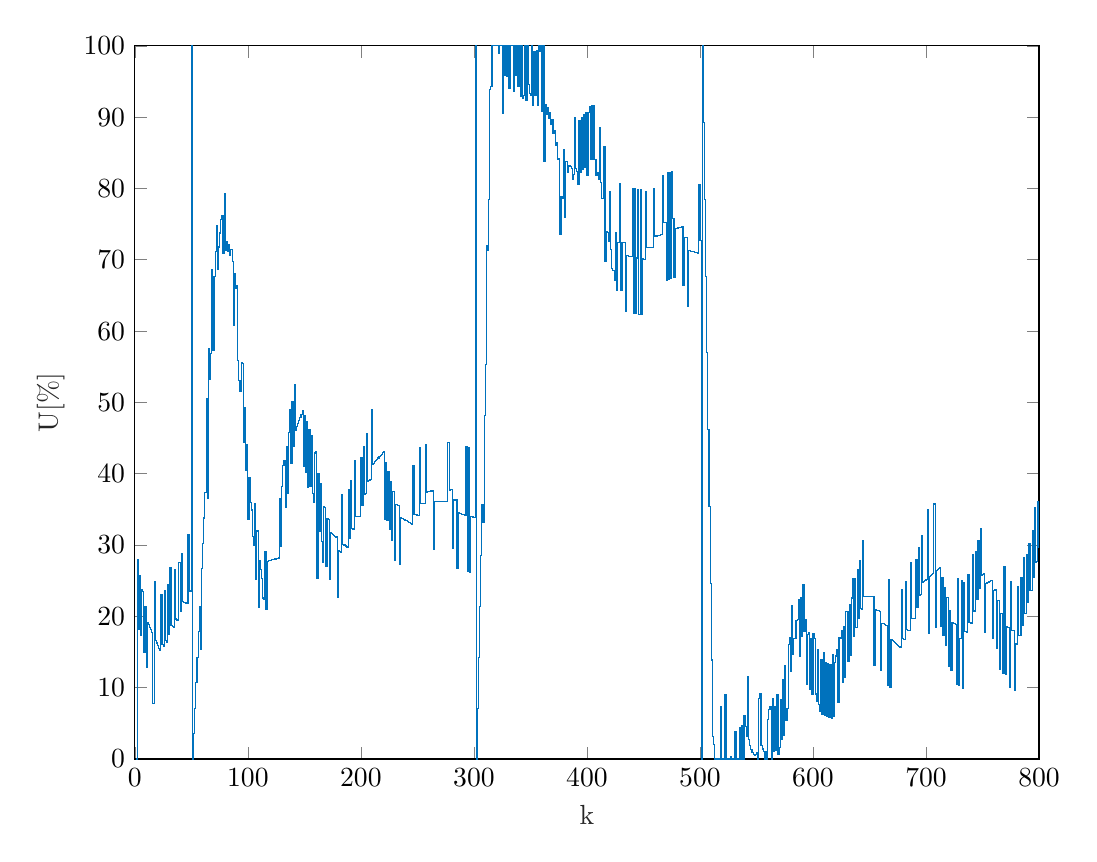
\begin{tikzpicture}

\begin{axis}[%
width=4.521in,
height=3.566in,
at={(0.758in,0.481in)},
scale only axis,
xmin=0,
xmax=800,
xlabel style={font=\color{white!15!black}},
xlabel={k},
ymin=0,
ymax=100,
ylabel style={font=\color{white!15!black}},
ylabel={U[\%]},
axis background/.style={fill=white}
]
\addplot[const plot, color=mycolor1, forget plot] table[row sep=crcr] {%
1	0\\
2	27.946429\\
3	18.117857\\
4	25.764286\\
5	17.264286\\
6	23.742857\\
7	23.471429\\
8	14.928571\\
9	21.364286\\
10	12.778571\\
11	19.171429\\
12	18.814286\\
13	18.457143\\
14	18.1\\
15	17.742857\\
16	7.735714\\
17	24.853571\\
18	16.621429\\
19	16.264286\\
20	15.907143\\
21	15.55\\
22	15.192857\\
23	23.107143\\
24	16.042857\\
25	15.728571\\
26	23.685714\\
27	16.664286\\
28	16.392857\\
29	24.392857\\
30	17.414286\\
31	26.835714\\
32	18.782143\\
33	18.603571\\
34	18.425\\
35	26.517857\\
36	19.632143\\
37	19.496429\\
38	19.360714\\
39	27.496429\\
40	20.653571\\
41	28.832143\\
42	22.032143\\
43	21.982143\\
44	21.932143\\
45	21.882143\\
46	21.832143\\
47	31.432143\\
48	23.557143\\
49	23.557143\\
50	100\\
51	0\\
52	3.571429\\
53	7.142857\\
54	10.714286\\
55	14.285714\\
56	17.857143\\
57	21.428571\\
58	15.35\\
59	26.746429\\
60	30.267857\\
61	33.789286\\
62	37.310714\\
63	50.482143\\
64	36.528571\\
65	57.575\\
66	53.271429\\
67	56.842857\\
68	68.685714\\
69	57.278571\\
70	67.6\\
71	71.171429\\
72	74.742857\\
73	68.664286\\
74	71.789286\\
75	73.746429\\
76	75.660714\\
77	76.153571\\
78	70.828571\\
79	79.314286\\
80	71.357143\\
81	72.560714\\
82	71.175\\
83	72.2\\
84	70.635714\\
85	71.482143\\
86	69.739286\\
87	60.757143\\
88	68.039286\\
89	65.982143\\
90	66.335714\\
91	55.828571\\
92	53.060714\\
93	51.535714\\
94	55.65\\
95	55.425\\
96	44.339286\\
97	49.264286\\
98	40.453571\\
99	44.032143\\
100	33.621429\\
101	39.475\\
102	35.989286\\
103	34.914286\\
104	31.25\\
105	29.996429\\
106	35.803571\\
107	25.167857\\
108	31.964286\\
109	21.192857\\
110	27.853571\\
111	26.596429\\
112	25.296429\\
113	22.575\\
114	22.307143\\
115	29.142857\\
116	20.957143\\
117	27.75\\
118	27.792857\\
119	27.835714\\
120	27.878571\\
121	27.921429\\
122	27.964286\\
123	28.007143\\
124	28.05\\
125	28.092857\\
126	28.135714\\
127	28.178571\\
128	36.492857\\
129	29.828571\\
130	38.185714\\
131	41.214286\\
132	41.789286\\
133	35.260714\\
134	43.753571\\
135	37.267857\\
136	45.803571\\
137	49.010714\\
138	41.492857\\
139	50.121429\\
140	43.771429\\
141	52.442857\\
142	46.135714\\
143	46.578571\\
144	47.021429\\
145	47.464286\\
146	47.907143\\
147	48.35\\
148	48.792857\\
149	40.964286\\
150	48.114286\\
151	40.242857\\
152	47.35\\
153	38.057143\\
154	46.239286\\
155	38.275\\
156	45.289286\\
157	37.282143\\
158	35.982143\\
159	42.910714\\
160	43.089286\\
161	25.346429\\
162	40.057143\\
163	31.871429\\
164	38.664286\\
165	30.435714\\
166	27.535714\\
167	35.360714\\
168	35.310714\\
169	26.989286\\
170	33.646429\\
171	33.553571\\
172	25.189286\\
173	31.803571\\
174	31.667857\\
175	31.532143\\
176	31.396429\\
177	31.260714\\
178	31.125\\
179	22.717857\\
180	29.289286\\
181	29.110714\\
182	28.932143\\
183	37.025\\
184	30.139286\\
185	30.003571\\
186	29.867857\\
187	29.732143\\
188	29.596429\\
189	37.732143\\
190	30.889286\\
191	39.067857\\
192	32.267857\\
193	32.217857\\
194	41.817857\\
195	33.942857\\
196	33.942857\\
197	33.942857\\
198	33.942857\\
199	33.942857\\
200	42.214286\\
201	35.507143\\
202	43.821429\\
203	37.157143\\
204	37.242857\\
205	45.6\\
206	38.978571\\
207	39.107143\\
208	39.235714\\
209	49.014286\\
210	41.317857\\
211	41.496429\\
212	41.675\\
213	41.853571\\
214	42.032143\\
215	42.210714\\
216	42.389286\\
217	42.567857\\
218	42.746429\\
219	42.925\\
220	43.103571\\
221	33.632143\\
222	41.635714\\
223	33.492857\\
224	40.328571\\
225	32.142857\\
226	38.935714\\
227	30.707143\\
228	37.457143\\
229	37.457143\\
230	27.807143\\
231	35.632143\\
232	35.582143\\
233	35.532143\\
234	27.210714\\
235	33.867857\\
236	33.775\\
237	33.682143\\
238	33.589286\\
239	33.496429\\
240	33.403571\\
241	33.310714\\
242	33.217857\\
243	33.125\\
244	33.032143\\
245	32.939286\\
246	41.117857\\
247	34.317857\\
248	34.267857\\
249	34.217857\\
250	34.167857\\
251	34.117857\\
252	43.717857\\
253	35.842857\\
254	35.842857\\
255	35.842857\\
256	35.842857\\
257	44.114286\\
258	37.407143\\
259	37.45\\
260	37.492857\\
261	37.535714\\
262	37.578571\\
263	37.621429\\
264	29.392857\\
265	36.142857\\
266	36.142857\\
267	36.142857\\
268	36.142857\\
269	36.142857\\
270	36.142857\\
271	36.142857\\
272	36.142857\\
273	36.142857\\
274	36.142857\\
275	36.142857\\
276	36.142857\\
277	44.414286\\
278	37.707143\\
279	37.75\\
280	37.792857\\
281	29.564286\\
282	36.314286\\
283	36.314286\\
284	36.314286\\
285	26.664286\\
286	34.489286\\
287	34.439286\\
288	34.389286\\
289	34.339286\\
290	34.289286\\
291	34.239286\\
292	34.189286\\
293	43.789286\\
294	26.264286\\
295	43.739286\\
296	26.214286\\
297	34.039286\\
298	33.989286\\
299	33.939286\\
300	33.889286\\
301	100\\
302	0\\
303	7.142857\\
304	14.285714\\
305	21.428571\\
306	28.571429\\
307	35.714286\\
308	33.207143\\
309	48.175\\
310	55.267857\\
311	72.010714\\
312	71.278571\\
313	78.421429\\
314	93.835714\\
315	94.271429\\
316	100\\
317	100\\
318	100\\
319	100\\
320	100\\
321	100\\
322	98.914286\\
323	100\\
324	100\\
325	90.55\\
326	100\\
327	95.792857\\
328	100\\
329	95.657143\\
330	100\\
331	93.957143\\
332	100\\
333	100\\
334	100\\
335	93.557143\\
336	100\\
337	95.832143\\
338	100\\
339	94.232143\\
340	100\\
341	92.885714\\
342	100\\
343	92.664286\\
344	93.067857\\
345	100\\
346	92.307143\\
347	100\\
348	94.582143\\
349	93.282143\\
350	92.971429\\
351	100\\
352	91.592857\\
353	99.196429\\
354	93.064286\\
355	99.321429\\
356	91.589286\\
357	100\\
358	99.192857\\
359	100\\
360	90.742857\\
361	100\\
362	83.814286\\
363	91.767857\\
364	90.382143\\
365	91.407143\\
366	89.842857\\
367	90.689286\\
368	88.946429\\
369	89.614286\\
370	87.692857\\
371	88.182143\\
372	86.082143\\
373	86.392857\\
374	84.114286\\
375	84.246429\\
376	73.517857\\
377	78.8\\
378	78.617857\\
379	85.496429\\
380	75.932143\\
381	83.8\\
382	83.75\\
383	82.278571\\
384	83.260714\\
385	83.075\\
386	82.846429\\
387	81.196429\\
388	82\\
389	89.907143\\
390	82.792857\\
391	82.385714\\
392	80.557143\\
393	89.453571\\
394	82.203571\\
395	89.932143\\
396	82.639286\\
397	90.325\\
398	82.989286\\
399	90.632143\\
400	81.875\\
401	90.592857\\
402	91.435714\\
403	84.007143\\
404	91.557143\\
405	84.085714\\
406	91.592857\\
407	84.078571\\
408	81.892857\\
409	82.160714\\
410	81.260714\\
411	88.589286\\
412	80.896429\\
413	78.532143\\
414	78.621429\\
415	85.814286\\
416	69.714286\\
417	73.921429\\
418	73.832143\\
419	72.575\\
420	79.546429\\
421	71.496429\\
422	68.775\\
423	68.507143\\
424	67.071429\\
425	73.864286\\
426	65.635714\\
427	72.385714\\
428	72.385714\\
429	80.657143\\
430	65.678571\\
431	72.428571\\
432	72.428571\\
433	72.428571\\
434	62.778571\\
435	70.603571\\
436	70.553571\\
437	70.503571\\
438	70.453571\\
439	70.403571\\
440	80.003571\\
441	62.478571\\
442	79.953571\\
443	62.428571\\
444	70.253571\\
445	79.853571\\
446	62.328571\\
447	79.803571\\
448	62.278571\\
449	70.103571\\
450	70.053571\\
451	70.003571\\
452	79.603571\\
453	71.728571\\
454	71.728571\\
455	71.728571\\
456	71.728571\\
457	71.728571\\
458	71.728571\\
459	80\\
460	73.292857\\
461	73.335714\\
462	73.378571\\
463	73.421429\\
464	73.464286\\
465	73.507143\\
466	73.55\\
467	81.864286\\
468	75.2\\
469	75.285714\\
470	67.1\\
471	82.164286\\
472	67.228571\\
473	82.292857\\
474	67.357143\\
475	82.421429\\
476	75.757143\\
477	67.571429\\
478	74.364286\\
479	74.407143\\
480	74.45\\
481	74.492857\\
482	74.535714\\
483	74.578571\\
484	74.621429\\
485	66.392857\\
486	73.142857\\
487	73.142857\\
488	73.142857\\
489	63.492857\\
490	71.317857\\
491	71.267857\\
492	71.217857\\
493	71.167857\\
494	71.117857\\
495	71.067857\\
496	71.017857\\
497	70.967857\\
498	70.917857\\
499	80.517857\\
500	72.642857\\
501	0\\
502	100\\
503	89.235714\\
504	78.471429\\
505	67.707143\\
506	56.942857\\
507	46.178571\\
508	35.414286\\
509	24.65\\
510	13.885714\\
511	3.121429\\
512	2.007143\\
513	0\\
514	0\\
515	0\\
516	0\\
517	0\\
518	7.292857\\
519	0\\
520	0\\
521	0\\
522	9.035714\\
523	0\\
524	0.010714\\
525	0\\
526	0\\
527	0.367857\\
528	0\\
529	0\\
530	0\\
531	3.803571\\
532	0\\
533	0\\
534	0\\
535	4.382143\\
536	0\\
537	4.696429\\
538	0\\
539	6.128571\\
540	4.560714\\
541	3.171429\\
542	11.610714\\
543	2.753571\\
544	1.95\\
545	1.325\\
546	0.878571\\
547	0.610714\\
548	0.521429\\
549	0.610714\\
550	0.878571\\
551	0\\
552	8.45\\
553	9.203571\\
554	1.864286\\
555	1.410714\\
556	1.092857\\
557	0\\
558	1.071429\\
559	0\\
560	5.546429\\
561	6.975\\
562	7.414286\\
563	0\\
564	8.535714\\
565	1.060714\\
566	7.321429\\
567	1.192857\\
568	9.053571\\
569	0.65\\
570	1.585714\\
571	8.382143\\
572	2.789286\\
573	11.185714\\
574	3.317857\\
575	13.060714\\
576	5.414286\\
577	7.107143\\
578	16.039286\\
579	16.978571\\
580	12.278571\\
581	21.567857\\
582	14.592857\\
583	16.957143\\
584	16.910714\\
585	19.453571\\
586	19.585714\\
587	22.307143\\
588	14.346429\\
589	22.575\\
590	17.246429\\
591	24.485714\\
592	17.914286\\
593	19.514286\\
594	10.389286\\
595	17.410714\\
596	17.725\\
597	9.810714\\
598	16.917857\\
599	9.046429\\
600	17.575\\
601	16.9\\
602	9.121429\\
603	8.092857\\
604	15.335714\\
605	7.6\\
606	6.614286\\
607	13.9\\
608	6.207143\\
609	14.914286\\
610	6.146429\\
611	13.525\\
612	5.925\\
613	13.346429\\
614	5.789286\\
615	13.253571\\
616	5.739286\\
617	14.625\\
618	6.035714\\
619	13.592857\\
620	14.442857\\
621	15.335714\\
622	8\\
623	17.064286\\
624	16.925\\
625	17.953571\\
626	10.753571\\
627	18.575\\
628	11.417857\\
629	20.660714\\
630	20.7\\
631	13.635714\\
632	21.592857\\
633	14.571429\\
634	22.571429\\
635	25.242857\\
636	17.189286\\
637	25.282143\\
638	18.396429\\
639	26.532143\\
640	19.689286\\
641	27.867857\\
642	21.067857\\
643	21.017857\\
644	30.617857\\
645	22.742857\\
646	22.742857\\
647	22.742857\\
648	22.742857\\
649	22.742857\\
650	22.742857\\
651	22.742857\\
652	22.742857\\
653	22.742857\\
654	13.092857\\
655	20.917857\\
656	20.867857\\
657	20.817857\\
658	20.767857\\
659	20.717857\\
660	12.396429\\
661	19.053571\\
662	18.960714\\
663	18.867857\\
664	18.775\\
665	18.682143\\
666	10.317857\\
667	25.203571\\
668	10.089286\\
669	16.703571\\
670	16.567857\\
671	16.432143\\
672	16.296429\\
673	16.160714\\
674	16.025\\
675	15.889286\\
676	15.753571\\
677	15.617857\\
678	23.753571\\
679	16.910714\\
680	16.817857\\
681	16.725\\
682	24.903571\\
683	18.103571\\
684	18.053571\\
685	18.003571\\
686	27.603571\\
687	19.728571\\
688	19.728571\\
689	19.728571\\
690	19.728571\\
691	28\\
692	21.292857\\
693	29.607143\\
694	22.942857\\
695	23.028571\\
696	31.385714\\
697	24.764286\\
698	24.892857\\
699	25.021429\\
700	25.15\\
701	34.928571\\
702	17.582143\\
703	25.585714\\
704	25.714286\\
705	25.842857\\
706	25.971429\\
707	35.75\\
708	18.403571\\
709	26.407143\\
710	26.535714\\
711	26.664286\\
712	26.792857\\
713	18.65\\
714	25.485714\\
715	17.3\\
716	24.092857\\
717	15.864286\\
718	22.614286\\
719	22.614286\\
720	12.964286\\
721	20.789286\\
722	12.467857\\
723	19.125\\
724	19.032143\\
725	18.939286\\
726	18.846429\\
727	10.482143\\
728	25.367857\\
729	10.253571\\
730	16.867857\\
731	25.003571\\
732	9.889286\\
733	24.775\\
734	17.932143\\
735	17.839286\\
736	17.746429\\
737	25.925\\
738	19.125\\
739	19.075\\
740	19.025\\
741	28.625\\
742	20.75\\
743	20.75\\
744	29.021429\\
745	22.314286\\
746	30.628571\\
747	23.964286\\
748	32.321429\\
749	25.7\\
750	25.828571\\
751	25.957143\\
752	17.814286\\
753	24.65\\
754	24.735714\\
755	24.821429\\
756	24.907143\\
757	24.992857\\
758	25.078571\\
759	16.892857\\
760	23.685714\\
761	23.728571\\
762	15.5\\
763	22.25\\
764	22.25\\
765	12.6\\
766	20.425\\
767	20.375\\
768	12.053571\\
769	26.982143\\
770	11.910714\\
771	18.567857\\
772	18.475\\
773	18.382143\\
774	10.017857\\
775	24.903571\\
776	18.060714\\
777	17.967857\\
778	9.603571\\
779	16.217857\\
780	16.082143\\
781	24.217857\\
782	17.375\\
783	17.282143\\
784	25.460714\\
785	18.660714\\
786	28.260714\\
787	20.385714\\
788	20.385714\\
789	28.657143\\
790	21.95\\
791	30.264286\\
792	23.6\\
793	23.685714\\
794	32.042857\\
795	25.421429\\
796	35.2\\
797	27.503571\\
798	27.682143\\
799	36.132143\\
800	29.603571\\
};
\end{axis}
\end{tikzpicture}%
\caption{Sterowanie PID z laboratorium 1}
\end{figure}

Wartość wskaźnika jakości:

\begin{equation}
E = 15451,8898
\end{equation}
